\subsection{\secState{R}Air Traffic Control}\label{sec:AirTrafficControl}
\paragraph{Motivation:} The modern \emph{Air Traffic Control} (ATC) procedures are outlined in ICAO 4444 \cite{icao4444}. The ATC roles and responsibilities in terms of \emph{clearance}, \emph{self-separation}, and, \emph{provided traffic information} are summarized in (tab. \ref{tab:airspaceResponsibilitiesIcao}). 

The \emph{main role} of \emph{Air Traffic Control} (ATC) is to support the organization of the \emph{airspace} in terms of \emph{preemptive} detect and avoid.

\begin{note}
    The \emph{Reactive} and \emph{Event Based} detect and avoid for manned aviation are covered by \emph{ACAS-X/TCAS systems} (sec. \ref{sec:ACASX}, \ref{sec:TCAS})
\end{note}

\paragraph{Commands issued by ATC:} There is multiple levels of commands issued by ATC, their characteristics and compulsory level is defined as folow:

\begin{enumerate}
    \item \emph{Notification} - the information notification, commonly known as \emph{NoTice to AirMan} (NOTAM), depending on flight mode, can be transmitted as voice message or information broadcast. They usually contains information about weather and traffic situation in given sector.
    
    \item \emph{Warning} - directed message to specific general aviation  which may require some direct action. The information is usually informative, but the action is not mandatory.
    
    \item \emph{Recommendation} - directed message to specific general aviation  which requires direct action. The order is usually specific action, but the action is not mandatory to be executed by pilot.
    
    \item \emph{Directive} - directed message to specific general aviation  which requires direct action. The order is specific action and the order fulfillment is mandatory for the pilot. 
\end{enumerate}

\paragraph{Separation enforcement:} The \emph{separation} is main feature of the ATC in controlled airspace of airports (B, C, D class). Its enforced by management of \emph{action clearance}. The ATC issues the clearance for take-off/landing sequence. 

The clearance for climb/descent is given at the beginning when flight plan is approved. The ATC issues the time slots for selected pathways. The continuous monitoring of air traffic is executed in periods. The airplane deviation from cleared plan should be minimal. 

If there is any incident the the \emph{ATC} can take following actions:
\begin{enumerate}
    
    \item \emph{Heading change} - order \emph{general aviation} to change heading in given time frame (horizontal navigation). This command is usually issued to correct horizontal deviations in path tracking.
    
    \item \emph{Velocity change} - order \emph{general aviation} to change velocity in given time frame. This command is usually issued to correct time deviations in path tracking.
    
    \item \emph{Altitude change} (Flight Level) - order \emph{general aviation} to climb or descent in given time frame. This command is usually issued to correct vertical deviations in path tracking (wrong flight level).
    
    \item \emph{Divergence} - order \emph{general aviation} to follow different waypoint in flight plan (goal change). This command is usually used to resolve incidents or to reroute traffic to other hub.
    
    \item \emph{Convergence} - order \emph{general aviation} to return to following original waypoint (goal return). This command is usually used when incident have been resolved in short time and original flight \emph{path} can be re-established.
    
    \item \emph{Restrictions Enforcement} - order \emph{general aviation} to avoid some point with defined distance.  
\end{enumerate}

\begin{note}
    All ATC commands can be requested be \emph{general aviation} for clearance to be granted. Meaning the airplane can ask ATC to perform any of listed actions. 
\end{note}

The \emph{separation} can be divined into two distinctive types to form \emph{well clear barrel} (fig. \ref{fig:WellClearTreshold}). The separation types are following:

\begin{enumerate}
    \item \emph{Horizontal separation} - keep clear of any intruders on horizontal plane (flight level plane).
    
    \item \emph{Vertical separation} - keep clear of any intruders on given altitude (flight level) range.
\end{enumerate}

\begin{note}
    The \emph{horizontal/vertical} separation is enforced independently, reducing 3D avoidance problem to 2D/1D avoidance problem.
\end{note}

\paragraph{Traffic Information:} The air traffic information is delivered to general aviation depending on airspace type (tab. \ref{tab:airspaceResponsibilitiesIcao}). 

\begin{note}
    The \emph{D class} airports usually do not have a radar or transponder therefore they can provide only visual guidance in altitude/horizontal range around "control tower".
\end{note}


\paragraph{Dynamic Airspace Management:} A real-time \emph{Airspace Management} approach have been presented in \cite{gardi2014real}. Following \emph{Dynamic Airspace Management} \cite{gerdes2016dynamic}. 

The \emph{airspace is usually} divided into the \emph{clusters} where each cluster is managed by separate ATC. When airplane is leaving one cluster, airplane hand-over is executed.

There is a problem when some airspace cluster is \emph{congested} or overloaded by controlled airplanes. The example of such situation is given in (fig. \ref{fig:DAMExample}). 

\begin{figure}[H]
    \centering
    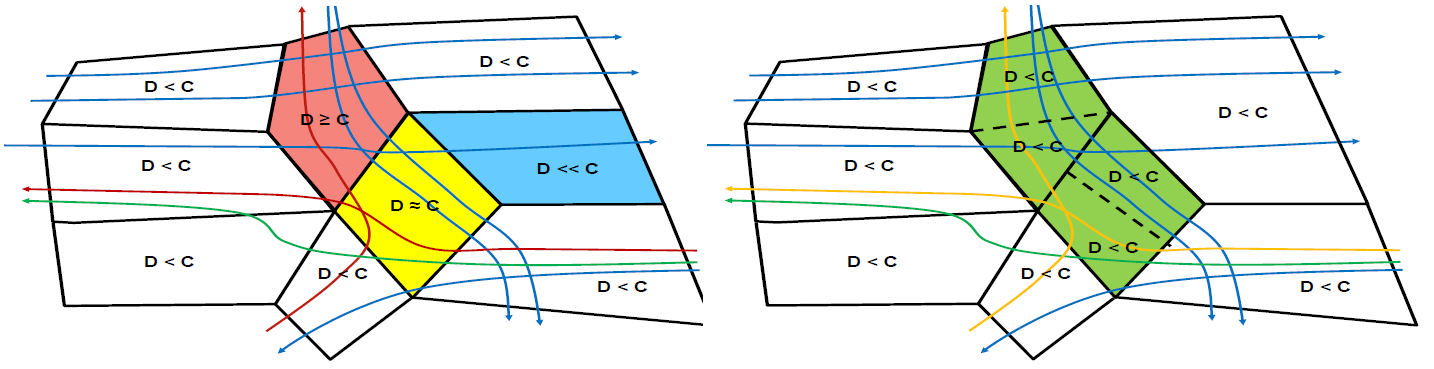
\includegraphics[width=1\textwidth]{\FIGDIR/02_02_DAM_Example}
    \caption{Example of DAM flight rerouting to homogenize traffic density \cite{gerdes2016dynamic}.}
    \label{fig:DAMExample}
\end{figure}

\begin{note}
    The air ways can not be changed, because the real time change of airways is difficult. The change of cluster authority is possible, because there is no changes for aircraft.
\end{note}

\noindent The airspace clusters are divined into three categories (fig. \ref{fig:DAMExample}):
\begin{enumerate}
    \item \emph{Under-fill} (blue) - there is less airplanes than its authority capacity.
    
    \item \emph{Saturated} (yellow) - there is enough airplanes to fill authority capacity.
    
    \item \emph{Over-fill} (red) - there is more airplanes than its authority capacity.
\end{enumerate}


\noindent The algorithm \cite{gerdes2016dynamic} will swap some airspace portions between neighbouring authorities to balance the load (all authorities should be saturated in ideal conditions) (green) (fig. \ref{fig:DAMExample}).